\begin{name}
	{\tenchude}
	{\tendethi}
	{\tentruong}
	{\thoigian}
\end{name}
\Opensolutionfile{ans}[ans/ans-De03HT]
% %==========Câu 1
% \begin{ex}%[1D2Y2-1]
% 	Trong mặt phẳng cho tập hợp $P$ gồm $10$ điểm phân biệt trong đó không có $3$ điểm nào thẳng hàng. Số tam giác có $3$ đỉnh đều thuộc tập hợp $P$ là
% 	\choice
% 	{\True $\mathrm{C}_{10}^{3}$}
% 	{$10^3$}
% 	{$\mathrm{A}_{10}^{3}$}
% 	{$\mathrm{C}_{7}^{3}$}
% 	\loigiai{Số tam giác có $3$ đỉnh đều thuộc tập hợp $P$ là $\mathrm{C}_{10}^3$.
% 	}
% \end{ex}
% %==========Câu 2
% \begin{ex}%[1D3Y3-3]
% 	Cho một cấp số cộng có $u_4=2$, $u_2=4$. Hỏi $u_1$ và công sai $d$ bằng bao nhiêu?
% 	\choice
% 	{$u_1=6$ và $d=1$}
% 	{$u_1=1$ và $d=1$}
% 	{\True $u_1=5$ và $d=-1$}
% 	{$u_1=-1$ và $d=-1$}
% 	\loigiai{Ta có $ u_n=u_1+ (n-1)d $. Theo giả thiết ta có hệ phương trình
% 	\[\left\{\begin{aligned}
% 	& u_4=2 \\
% 	& u_2=4
% 	\end{aligned}\right.\Leftrightarrow \left\{\begin{aligned}
% 	& u_1+3d=2 \\
% 	& u_1+d=4
% 	\end{aligned}\right.\Leftrightarrow \left\{\begin{aligned}
% 	& u_1=5 \\
% 	& d=-1.
% 	\end{aligned}\right.\]
% 	Vậy $u_1=5$ và $d=-1$.
% 	}
% \end{ex}
% %%==========Câu 3
% \begin{ex}%[2D1Y1-2]
% 	Cho hàm số $f(x)$ có bảng biến thiên như hình sau
% 	\begin{center}
% 	\begin{tikzpicture}
% 	\tkzTabInit[nocadre=true,lgt=1,espcl=2,deltacl=0.5]
% 	{$ x $ /.6, $ y' $ /.6, $ y $ /2} 	
% 	{$ -\infty $, $ -1 $, $ 0 $, $ 1 $, $ + \infty $}
% 	\tkzTabLine{,+, $ 0 $,-, $ 0 $,+, $ 0 $,-}
% 	\tkzTabVar{-/ $ -\infty $,+/ $ 2 $,-/ $ -1 $,+/ $ 2 $,-/ $ -\infty $}	
% 	\end{tikzpicture}
% 	\end{center}
% Hàm số đã cho nghịch biến trên khoảng nào dưới đây?
% 	\choice
% 	{$ (-\infty;-1)$}
% 	{$ (0;1)$}
% 	{\True $ (-1;0)$}
% 	{$ (-\infty;0)$}
% 	\loigiai{
% 	Dựa vào bảng biến thiên ta thấy $f'(x)<0$ trên các khoảng $ (-1;0)$ và $ (1;+\infty)$.\\
% 	Vậy hàm số nghịch biến trên $ (-1;0)$.
% 	}
% \end{ex}
% %%==========Câu 4
% \begin{ex}%[2D1Y2-2]
% 	Cho hàm số $ f(x) $ có bảng biến thiên như hình sau 
% 	\begin{center}
% 	\begin{tikzpicture}
% 	\tkzTabInit[nocadre=true,lgt=1,espcl=2,deltacl=0.5]
% 	{$ x $ /.6, $ y' $ /.6, $ y $ /2} 	
% 	{$ -\infty $, $ -1 $, $ 0 $, $ 1 $, $ + \infty $}
% 	\tkzTabLine{,+, $ 0 $,-, $ 0 $,+, $ 0 $,-}
% 	\tkzTabVar{-/ $ -\infty $,+/ $ 1 $,-/ $ 0 $,+/ $ 1 $,-/ $ -\infty $}	
% 	\end{tikzpicture}
% 	\end{center}
% Hàm số đã cho đạt cực tiểu tại
% 	\choice
% 	{$ x=-1 $}
% 	{$ x=1 $}
% 	{\True $ x=0 $}
% 	{$ x=2 $}
% 	\loigiai{Theo bảng biến thiên ta thấy hàm số đạt cực tiểu tại $x=0$.
% 	}
% \end{ex}
% %==========Câu 5
% \begin{ex}%[2D1Y2-2]
% 	Cho hàm số $ y=f(x) $ có bảng biến thiên như hình sau 
% 	\begin{center}
% 	\begin{tikzpicture}
% 	\tkzTabInit[nocadre=true,lgt=1,espcl=2,deltacl=0.5]
% 	{$ x $ /.6, $ y' $ /.6, $ y $ /2} 	
% 	{$ -\infty $, $ 0 $, $ 2 $, $ + \infty $}
% 	\tkzTabLine{,+, $ 0 $,-, $ 0 $,+}
% 	\tkzTabVar{-/ $ -\infty $,+/ $ 5 $,-/ $ 1 $,+/ $ +\infty $}
% 	\end{tikzpicture}
% 	\end{center}
% Mệnh đề nào dưới đây đúng?
% 	\choice
% 	{Hàm số không có cực trị}
% 	{\True Hàm số đạt cực đại tại $ x=0 $}
% 	{Hàm số đạt cực đại tại $ x=5 $}
% 	{Hàm số đạt cực tiểu tại $ x=1 $}
% 	\loigiai{Từ bảng biến thiên ta thấy hàm số đạt cực đại bằng $ 5 $ tại $ x=0 $.
% 	}
% \end{ex}
% %%==========Câu 6
% \begin{ex}%[2D1Y4-1]
% 	Tiệm cận đứng của đồ thị hàm số $ y=\dfrac{2-x}{x+3} $ là
% 	\choice
% 	{$ x=2 $}
% 	{\True $ x=-3 $}
% 	{$ y=-1 $}
% 	{$ y=-3 $}
% 	\loigiai{Tập xác định của hàm số $\mathscr{D}=\mathbb{R}\setminus  \{-3 \} $.\\
% 	Ta có $ \displaystyle\lim\limits_{x\to{ (-3)^{+}}} y=\displaystyle\lim\limits_{x\to{ (-3)^{+}}}\dfrac{2-x}{x+3}=+\infty $.\\
% 	Suy ra đồ thị hàm số đã cho có tiệm cận đứng là đường thẳng $ x=-3 $.
% 	}
% \end{ex}
% %%==========Câu 7
% \begin{ex}%[2D1Y5-1]
% \immini{Đồ thị của hàm số nào dưới đây có dạng như đường cong trong hình bên?
% 	\choice
% 	{$ y=-x^2+x-1 $}
% 	{$ y=-x^3+3x+1 $}
% 	{$ y=x^4-x^2+1 $}
% 	{\True $ y=x^3-3x+1 $}
% 	}
% 	{
% 	\begin{tikzpicture}[line join = round, line cap = round,>=stealth,scale=0.7]
% 	\def\f(#1){(#1)^3-3*(#1)+1} %định nghĩa hàm số
% 	\draw[->](-3,0)--(3,0) node[below] {$x$};
% 	\draw[->](0,-2)--(0,3.5) node[left] {$y$};
% 	\draw[smooth,samples=100] plot[domain=-2.1:2.02](\x,{\f(\x)});
% 	\draw[fill=black] (0,0) node[below left] {$O$} circle (1pt);
% 	\end{tikzpicture}
% 	}
% 	\loigiai{Đặc trưng của đồ thị là hàm bậc ba nên loại đáp án $ y=-x^2+x-1 $ và $ y=x^4-x^2+1 $.\\
% 	Lại có $ \displaystyle\lim\limits_{x\to +\infty}y=+\infty $ nên $ a>0 $ do đó đồ thị hàm số cần tìm là $ y=x^3-3x+1 $.
% 	}
% \end{ex}
% %%==========Câu 8
% \begin{ex}%[2D1Y5-4]
% 	Đồ thị hàm số $y=-x^4+x^2+2$ cắt trục $Oy$ tại điểm
% 	\choice
% 	{\True $A (0;2)$}
% 	{$A (2;0)$}
% 	{$A (0;-2)$}
% 	{$A (0;0)$}
% 	\loigiai{Với $x=0\Rightarrow y=2$. Vậy đồ thị hàm số $y=-x^4+x^2+2$ cắt trục $Oy$ tại điểm $A (0;2)$.
% 	}
% \end{ex}
% %%%=========HetCau_8=========%%%
% %%==========Câu 9
% \begin{ex}%[2D2Y3-2]
% 	Cho $ a $ là số thực dương bất kì. Tìm khẳng định đúng trong các khẳng định sau
% 	\choice
% 	{$ \log a^3=\dfrac{1}{3}\log a $}
% 	{$ \log  (3a)=3\log a $}
% 	{$ \log  (3a)=\dfrac{1}{3}\log a $}
% 	{\True $ \log a^3=3\log a $}
% 	\loigiai{
% 	Ta có $ \log a^3=3\log a $.
% 	}
% \end{ex}
% %%%=========HetCau_9=========%%%
% %%==========Câu 10
% \begin{ex}%[1D5Y2-1]
% 	Đạo hàm của hàm số $ y=6^x $ là
% 	\choice
% 	{$ y'=6^x $}
% 	{\True $ y'=6^x\ln 6 $}
% 	{$ y'=\dfrac{6^x}{\ln 6} $}
% 	{$ y'=x\cdot 6^{x-1} $}
% 	\loigiai{Ta có $ y=6^x\Rightarrow y'=6^x\ln 6 $.
% 	}
% \end{ex}
% %%%=========HetCau_10=========%%%
% %%==========Câu 11
% \begin{ex}%[2D2Y1-2]
% 	Cho số thực dương $ x $. Viết biểu thức $ P=\sqrt[3]{x^5}\cdot \dfrac{1}{\sqrt{x^3}} $ dưới dạng lũy thừa cơ số $ x $ ta được kết quả 
% 	\choice
% 	{$ P=x^{\frac{19}{15}} $}
% 	{$ P=x^{\frac{19}{6}} $}
% 	{\True $P=x^{\frac{1}{6}} $}
% 	{$ P=x^{-\frac{1}{15}} $}
% 	\loigiai{
% 	Ta có $P=\sqrt[3]{x^5}\cdot\dfrac{1}{\sqrt{x^3}}=x^{\tfrac{5}{3}}\cdot x^{-\frac{3}{2}}=x^{\frac{5}{3}-\frac{3}{2}}=x^{\frac{1}{6}}$.
% 	}
% \end{ex}
% %%%=========HetCau_11=========%%%
% %%==========Câu 12
% \begin{ex}%[2D2Y5-1]
% 	Nghiệm của phương trình $2^{x-1}=\dfrac{1}{16}$ là
% 	\choice
% 	{\True $ x=-3 $}
% 	{$ x=5 $}
% 	{$ x=4 $}
% 	{$ x=3 $}
% 	\loigiai{
% 	Phương trình đã cho $ \Leftrightarrow{2^{x-1}}=2^{-4}\Leftrightarrow x-1=-4\Leftrightarrow x=-3$.
% 	}
% \end{ex}
% %%%=========HetCau_12=========%%%
% %%==========Câu 13
% \begin{ex}%[2D2Y5-1]
% 	Nghiệm của phương trình $ \log_4(3x-2)=2 $ là
% 	\choice
% 	{\True $ x=6 $}
% 	{$ x=3 $}
% 	{$ x=\dfrac{10}{3} $}
% 	{$ x=\dfrac{7}{2} $}
% 	\loigiai{Ta có $ \log_4(3x-2)=2\Leftrightarrow 3x-2=4^2\Leftrightarrow 3x-2=16\Leftrightarrow x=6 $.
% 	}
% \end{ex}
% %%%=========HetCau_13=========%%%
% %%==========Câu 14
% \begin{ex}%[2D3Y1-1]
% 	Họ nguyên hàm của hàm số $ f(x)=3x^2+\sin x $ là
% 	\choice
% 	{$ x^3+\cos x+C $}
% 	{$ 6x+\cos x+C $}
% 	{\True $ x^3-\cos x+C $}
% 	{$ 6x-\cos x+C $}
% 	\loigiai{Ta có $ \displaystyle\int (3x^2+\sin x)\mathrm{\,d}x=x^3-\cos x+C $.
% 	}
% \end{ex}
% %%%=========HetCau_14=========%%%
% %%==========Câu 15
% \begin{ex}%[2D3Y1-1]
% 	Tìm họ nguyên hàm của hàm số $ f(x)=\mathrm{e}^{3x} $.
% 	\choice
% 	{$ \displaystyle\int{f(x)\mathrm{\,d}x=\dfrac{\mathrm{e}^{3x+1}}{3x+1}}+C $}
% 	{$ \displaystyle\int{f(x)\mathrm{\,d}x=3\mathrm{e}^{3x}}+C $}
% 	{$ \displaystyle\int{f(x)\mathrm{\,d}x=\mathrm{e}^3}+C $}
% 	{\True $ \displaystyle\int{f(x)\mathrm{\,d}x=\dfrac{\mathrm{e}^{3x}}{3}}+C $}
% 	\loigiai{Ta có $ \displaystyle\int{\mathrm{e}^{3x}\mathrm{\,d}x=\dfrac{\mathrm{e}^{3x}}{3}}+C $.
% 	}
% \end{ex}
% %%%=========HetCau_15=========%%%
% %%==========Câu 16
% \begin{ex}%[2D3B2-1]
% 	Cho hàm số $ f(x) $ liên tục trên $ \mathbb{R} $ thỏa mãn $ \displaystyle\int\limits_0^6f(x)\mathrm{\,d}x=7 $, $ \displaystyle\int\limits_6^{10}f(x)\mathrm{\,d}x=-1 $. Giá trị của $ I=\displaystyle\int\limits_0^{10}f(x)\mathrm{\,d}x $ bằng
% 	\choice
% 	{$ I=5 $}
% 	{\True $ I=6 $}
% 	{$ I=7 $}
% 	{$ I=8 $}
% 	\loigiai{Ta có $ I=\displaystyle\int\limits_0^{10}f(x)\mathrm{\,d}x=\displaystyle\int\limits_0^6f(x)\mathrm{\,d}x+\displaystyle\int\limits_6^{10}f(x)\mathrm{\,d}x=7-1=6 $.\\
% 	Vậy $ I=6 $ 
% 	}
% \end{ex}
% %%%=========HetCau_16=========%%%
% %%==========Câu 17
% \begin{ex}%[2D3Y2-1]
% 	Giá trị của $\displaystyle\int\limits_0^{\tfrac{\pi}{2}}\sin x\mathrm{\,d}x $ bằng
% 	\choice
% 	{$ 0 $}
% 	{\True $ 1 $}
% 	{$ -1 $}
% 	{$ \dfrac{\pi}{2} $}
% 	\loigiai{Ta có $ \displaystyle\int\limits_0^{\tfrac{\pi}{2}}\sin x\mathrm{\,d}x=-\cos x\bigg|_0^{\tfrac{\pi}{2}}=1 $.
% 	}
% \end{ex}
% %%%=========HetCau_17=========%%%
% %%==========Câu 18
% \begin{ex}%[2D4Y1-1]
% 	Số phức liên hợp của số phức $ z=2+i $ là
% 	\choice
% 	{$ \overline{z}=-2+i $}
% 	{$ \overline{z}=-2-i $}
% 	{\True $ \overline{z}=2-i $}
% 	{$ \overline{z}=2+i $}
% 	\loigiai{Số phức liên hợp của số phức $ z=2+i $ là $ \overline{z}=2-i $.
% 	}
% \end{ex}
% %%%=========HetCau_18=========%%%
% %%==========Câu 19
% \begin{ex}%[2D4Y2-2]
% 	Cho hai số phức $ z_1=2+i $ và $ z_2=1+3i $. Phần thực của số phức $ z_1+z_2 $ bằng
% 	\choice
% 	{$ 1 $}
% 	{\True $ 3 $}
% 	{$ 4 $}
% 	{$ -2 $}
% 	\loigiai{Ta có $ z_1+z_2=(2+i)+(1+3i)=3+4i $. Vậy phần thực của số phức $ z_1+z_2 $ bằng $ 3 $.
% 	}
% \end{ex}
% %%%=========HetCau_19=========%%%
% %%==========Câu 20
% \begin{ex}%[2D4Y1-2]
% 	Trên mặt phẳng tọa độ, điểm biểu diễn số phức $ z=-1+2i $ là điểm nào dưới đây?
% 	\choice
% 	{$ Q(1; 2) $}
% 	{\True $ P(-1; 2) $}
% 	{$ N(1; -2) $}
% 	{$ M(-1;-2) $}
% 	\loigiai{Điểm biểu diễn số phức $ z=-1+2i $ là điểm $ P (-1; 2) $.
% 	}
% \end{ex}
% %%%=========HetCau_20=========%%%
% %%==========Câu 21
% \begin{ex}%[2H1Y3-2]
% 	Thể tích của khối lập phương cạnh $ 2 $ bằng
% 	\choice
% 	{$ 6 $}
% 	{\True $ 8 $}
% 	{$ 4 $}
% 	{$ 2 $}
% 	\loigiai{Ta có $ V=2^3=8 $.
% 	}
% \end{ex}
% %%%=========HetCau_21=========%%%
% %%==========Câu 22
% \begin{ex}%[2H1Y3-2]
% 	Cho khối chóp có thể tích bằng $32$ cm$^3$ và diện tích đáy bằng $16$ cm$^2$. Chiều cao của khối chóp đó là
% 	\choice
% 	{$ 4 $ cm}
% 	{\True $ 6 $ cm}
% 	{$ 3 $ cm}
% 	{$ 2 $ cm}
% 	\loigiai{Ta có $ V_{\text{chóp}}=\dfrac{1}{3}B\cdot h\Rightarrow h=\dfrac{3V}{B}=\dfrac{3\cdot 32}{16}=6 $ cm.
% 	}
% \end{ex}
% %%%=========HetCau_22=========%%%
% %%==========Câu 23
% \begin{ex}%[2H2Y1-1]
% 	Cho khối nón có chiều cao $ h=3 $ và bán kính đáy $ r=4 $. Thể tích của khối nón đã cho bằng
% 	\choice
% 	{\True $ 16\pi $}
% 	{$ 48\pi $}
% 	{$ 36\pi $}
% 	{$ 4\pi $}
% 	\loigiai{Thể tích của khối nón đã cho là $ V=\dfrac{1}{3}\pi r^2h=\dfrac{1}{3}\pi{4^2}\cdot 3=16\pi $.
% 	}
% \end{ex}
% %%%=========HetCau_23=========%%%
% %%==========Câu 24
% \begin{ex}%[2H2Y1-1]
% 	Tính theo $ a $ thể tích của một khối trụ có bán kính đáy là $ a $, chiều cao bằng $ 2a $ 
% 	\choice
% 	{\True $ 2\pi a^3 $}
% 	{$ \dfrac{2\pi a^3}{3} $}
% 	{$ \dfrac{\pi a^3}{3} $}
% 	{$ \pi a^3 $}
% 	\loigiai{Thể tích khối trụ là $ V=\pi\cdot R^2\cdot h=\pi\cdot a^2\cdot 2a=2\pi a^3 $.
% 	}
% \end{ex}
% %%%=========HetCau_24=========%%%
% %%==========Câu 25
% \begin{ex}%[2H3Y1-1]
% 	Trong không gian $ Oxyz $, cho $ A(2;-3;-6) $, $ B(0;5;2) $. Toạ độ trung điểm $ I $ của đoạn thẳng $ AB $ là
% 	\choice
% 	{$ I(-2;8;8) $}
% 	{\True $ I(1;1;-2) $}
% 	{$ I(-1;4;4) $}
% 	{$ I(2;2;-4) $}
% 	\loigiai{Vì $ I $ là trung điểm của $ AB $ nên $ I\left(\dfrac{x_A+x_B}{2};\dfrac{y_A+y_B}{2};\dfrac{z_A+z_B}{2}\right) $. Vậy $ I(1;1;-2) $.
% 	}
% \end{ex}
% %%%=========HetCau_25=========%%%
% %%==========Câu 26
% \begin{ex}%[2H2Y2-1]
% 	Trong KG $Oxyz$, cho mặt cầu $(S)\colon (x-2)^2+(y+4)^2+(z-1)^2=9$. Tâm của $(S)$ có tọa độ là
% 	\choice
% 	{$ (-2; 4;-1) $}
% 	{\True $ (2;-4; 1) $}
% 	{$ (2;4;1) $}
% 	{$ (-2;-4;-1) $}
% 	\loigiai{Mặt cầu $ (S) $ có tâm là $  (2;-4;1) $. 
% 	}
% \end{ex}
% %%%=========HetCau_26=========%%%
% %%==========Câu 27
% \begin{ex}%[2H3Y2-4]
% 	Trong không gian $ Oxyz $, cho mặt phẳng $(P)\colon x-2y+z-1=0 $. Điểm nào dưới đây thuộc $ (P) $?
% 	\choice
% 	{$ M(1;-2;1) $}
% 	{\True $ N(2;1;1) $}
% 	{$ P(0;-3;2) $}
% 	{$ Q(3;0;-4) $}
% 	\loigiai{Lần lượt thay toạ độ các điểm $ M $, $ N $, $ P $, $ Q $ vào phương trình $ (P) $, ta thấy toạ độ điểm $ N $ thoả mãn phương trình $ (P) $. Do đó điểm $ N $ thuộc $ (P) $.}
% \end{ex}
% %%%=========HetCau_27=========%%%
% %%==========Câu 28
% \begin{ex}%[2H3Y3-1]
% 	Trong không gian với hệ trục tọa độ $ Oxyz $, tìm một vectơ chỉ phương của đường thẳng \[ d\colon \left\{\begin{aligned}
% 	& x=4+7t \\
% 	& y=5+4t \\
% 	& z=-7-5t
% \end{aligned}\right. (t\in \mathbb{R}).\]
% 	\choice
% 	{$ \vec{u}_1=(7;-4;-5) $}
% 	{$ \vec{u}_2=(5;-4;-7) $}
% 	{$ \vec{u}_3=(4;5;-7) $}
% 	{\True $ \vec{u}_4=(7;4;-5) $}
% 	\loigiai{Vectơ chỉ phương của đường thẳng $ d $ là $ \vec{u}_4=(7;4;-5)$. 
% 	}
% \end{ex}
% %%%=========HetCau_28=========%%%
% %%==========Câu 29
% \begin{ex}%[1D2Y5-2]
% 	Một hội nghị có $ 15 $ nam và $ 6 $ nữ. Chọn ngẫu nhiên $ 3 $ người vào ban tổ chức. Xác suất để $ 3 $ người lấy ra là nam
% 	\choice
% 	{$ \dfrac{1}{2} $}
% 	{\True $ \dfrac{91}{266} $}
% 	{$ \dfrac{4}{33} $}
% 	{$ \dfrac{1}{11} $}
% 	\loigiai{
% 	Không gian mẫu là một tổ hợp chập $ 3 $ của $ 1 $ nên số phần tử là $ n (\Omega)=\mathrm{C}_{21}^{3}=1330$.\\
% 	Gọi $ A $ là biến cố: \lq\lq  $3$ người lấy ra là nam\rq\rq. Khi đó, $ n(A)=\mathrm{C}_{15}^3=455 $.\\
% 	Vậy xác suất để $3$ người lấy ra là nam là $ P(A)=\dfrac{n(A)}{n (\Omega)}=\dfrac{13}{38}=\dfrac{91}{266}$.
% 	}
% \end{ex}
% %%%=========HetCau_29=========%%%
% %%==========Câu 30
% \begin{ex}%[2D1B1-1]
% 	Trong các hàm số sau, hàm số nào đồng biến trên $ \mathbb{R} $?
% 	\choice
% 	{\True $ f(x)=x^3-3x^2+3x-4 $}
% 	{$ f(x)=x^2-4x+1 $}
% 	{$ f(x)=x^4-2x^2-4 $}
% 	{$ f(x)=\dfrac{2x-1}{x+1} $}
% 	\loigiai{Xét các phương án
% 	\begin{itemize}
% 	\item Hàm số $ f(x)=x^3-3x^2+3x-4\Rightarrow f'(x)=3x^2-6x+3=3(x-1)^2\ge 0 $, $ \forall x\in \mathbb{R} $ và dấu bằng xảy ra tại $ x=1 $. Do đó hàm số $ f(x)=x^3-3x^2+3x-4 $ đồng biến trên $ \mathbb{R} $.
% 	\item Hàm số $ f(x)=x^2-4x+1 $ là hàm bậc hai và luôn có một cực trị nên không đồng biến trên $ \mathbb{R} $.
% 	\item Hàm số $ f(x)=x^4-2x^2-4 $ là hàm trùng phương luôn có ít nhất một cực trị nên không đồng biến trên $ \mathbb{R} $.
% 	\item Hàm số $ f(x)=\dfrac{2x-1}{x+1} $ có $ \mathscr{D}=\mathbb{R}\setminus \{-1\} $ nên không đồng biến trên $\mathbb{R}$.
% 	\end{itemize}
% 	}
% \end{ex}
% %%%=========HetCau_30=========%%%
% %%==========Câu 31
% \begin{ex}%[2D1B3-1]
% 	Gọi $ M $, $ m $ lần lượt là giá trị lớn nhất, giá trị nhỏ nhất của hàm số $ y=x^4-10x^2+2 $ trên đoạn $ [-1;2] $. Tổng $ M+m $ bằng
% 	\choice
% 	{$ -27 $}
% 	{$ -29 $}
% 	{\True $ -20 $}
% 	{$ -5 $}
% 	\loigiai{Xét trên đoạn $ [-1;2] $.\\
% 	Ta có $ y'=4x^3-20x=4x (x^2-5) $.\\
% 	 $ y'=0\Leftrightarrow \left[\begin{aligned}
% 	& x=0 \in [-1;2] \\
% 	& x=\sqrt{5}\notin [-1;2]\\
% 	& x=-\sqrt{5}\notin [-1;2].
% \end{aligned}\right.$\\
% 	Lại có $ f(-1)=-7 $; $ f(0)=2 $; $ f(2)=-22 $.\\
% 	Do đó $ M=\max\limits_{[-1;2]} y=2 $, $ m=\min\limits_{[-1;2]} y=-22 $ nên $ M+m=-20 $.
% 	}
% \end{ex}
% %%%=========HetCau_31=========%%%
% %%==========Câu 32
% \begin{ex}%[2D2Y6-1]
% 	Tập nghiệm của bất phương trình $ \log x\ge 1 $ là
% 	\choice
% 	{$ (10;+\infty) $}
% 	{$ (0;+\infty) $}
% 	{\True $ [10; +\infty) $}
% 	{$ (-\infty;10) $}
% 	\loigiai{Ta có $ \log x\ge 1\Leftrightarrow x\ge 10 $.\\
% 	Vậy tập nghiệm của bất phương trình là $ [10; +\infty) $.
% 	}
% \end{ex}
% %%%=========HetCau_32=========%%%
% %%==========Câu 33
% \begin{ex}%[2D3Y2-1]
% 	Nếu $ \displaystyle\int\limits_0^1f(x)\mathrm{\,d}x=4 $ thì $ \displaystyle\int\limits_0^12f(x)\mathrm{\,d}x $ bằng
% 	\choice
% 	{$16$}
% 	{$4$}
% 	{$2$}
% 	{\True $8$}
% 	\loigiai{Ta có $\displaystyle\int\limits_{0}^{1} 2f(x)\mathrm{\,d}x=2\displaystyle\int\limits_{0}^{1} f(x)\mathrm{\,d}x=2\cdot 4=8$.
% 	}
% \end{ex}
% %%%=========HetCau_33=========%%%
% %%==========Câu 34
% \begin{ex}%[2D4Y1-1]
% 	Tính môđun số phức nghịch đảo của số phức $ z=(1-2i)^2 $.
% 	\choice
% 	{$ \dfrac{1}{\sqrt{5}} $}
% 	{$ \sqrt{5} $}
% 	{$ \dfrac{1}{25} $}
% 	{\True $ \dfrac{1}{5} $}
% 	\loigiai{Ta có $ z=(1-2i)^2=-3-4i $.\\
% 	Suy ra $ \dfrac{1}{z}=\dfrac{1}{-3-4i}=-\dfrac{3}{25}+\dfrac{4}{25}i $.\\
% 	Nên $ \left| \dfrac{1}{z} \right|=\sqrt{\left(\dfrac{-3}{25}\right)^2+\left(\dfrac{4}{25}\right)^2}=\dfrac{1}{5} $.
% 	}
% \end{ex}
% %%%=========HetCau_34=========%%%
% %%==========Câu 35
% \begin{ex}%[1H3Y3-3]
% \immini{Cho hình chóp $ S. ABC $ có $ SA $ vuông góc với mặt phẳng $ (ABC) $, $ SA=\sqrt{2}a $, tam giác $ ABC $ vuông cân tại $ B $ và $ AC=2a $ (minh họa như hình bên). Góc giữa đường thẳng $ SB $ và mặt phẳng $ (ABC) $ bằng
% 	\choice
% 	{$ 30^\circ $}
% 	{\True $ 45^\circ $}
% 	{$ 60^\circ $}
% 	{$ 90^\circ $}}{\begin{tikzpicture}[line join = round, line cap = round,>=stealth,scale=0.7]
% 	\path
% 	(0,0) coordinate(A)
% 	(2,-1.5) coordinate(B)
% 	(5,0)coordinate(C)
% 	;
% 	\coordinate (S) at ($ (A)+(0,4) $);
% 	\draw (S)--(A) (S)--(B) (S)--(C) (B)--(C) (A)--(B);
% 	\draw[dashed] (A)--(C);
% 	\foreach \d/\g in{A/180,B/-90,C/-90,S/90}\draw[fill=black](\d)circle(1pt)+(\g:0.35)node{$ \d $};
% 	\tkzMarkSegment[pos=0.5,mark=||](A,B)
% 	\tkzMarkSegment[pos=0.5,mark=||](B,C)
% 	\draw
% 	pic[draw, angle radius=2mm] {right angle=S--A--C}
% 	pic[draw, angle radius=2mm] {right angle=A--B--C}
% 	pic[draw, angle radius=2mm] {right angle=S--A--B};
% 	\end{tikzpicture}}
% 	\loigiai{
% 	\immini{Ta có $ SB\cap (ABC)=B $; $ SA\perp (ABC) $ tại $ A $.\\
% 	Nên hình chiếu vuông góc của $ SB $ lên mặt phẳng $ (ABC) $ là $ AB $.\\
% 	Do đó góc giữa đường thẳng $ SB $ và mặt phẳng $ (ABC) $ là $ \alpha=\widehat{SBA} $.\\
% 	Do tam giác $ ABC $ vuông cân tại $ B $ và $ AC=2a $ nên \[AB=\dfrac{AC}{\sqrt{2}}=\sqrt{2}a=SA.\] Suy ra tam giác $ SAB $ vuông cân tại $ A $.\\
% 	Do đó $ \alpha=\widehat{SBA}=45^\circ $.
% }
% {\begin{tikzpicture}[line join = round, line cap = round,>=stealth,scale=0.7]
% 	\path
% 	(0,0) coordinate(A)
% 	(2,-1.5) coordinate(B)
% 	(5,0)coordinate(C)
% 	;
% 	\coordinate (S) at ($ (A)+(0,4) $);
% 	\draw (S)--(A) (S)--(B) (S)--(C) (B)--(C) (A)--(B);
% 	\draw[dashed] (A)--(C);
% 	\foreach \d/\g in{A/180,B/-90,C/-90,S/90}\draw[fill=black](\d)circle(1pt)+(\g:0.35)node{$ \d $};
% 	\tkzMarkSegment[pos=0.5,mark=||](A,B)
% 	\tkzMarkSegment[pos=0.5,mark=||](B,C)
% 	\draw
% 	pic[draw, angle radius=2mm] {right angle=S--A--C}
% 	pic[draw, angle radius=2mm] {right angle=A--B--C}
% 	pic[draw, angle radius=2mm] {right angle=S--A--B}
% 	pic[draw, angle radius=5mm] {angle=S--B--A}
% 	;
% 	\end{tikzpicture}}
% 	\noindent Vậy góc giữa đường thẳng $ SB $ và mặt phẳng $ (ABC) $ bằng $ 45^\circ $.
% 	}
% \end{ex}
% %%%=========HetCau_35=========%%%
% %%==========Câu 36
% \begin{ex}%[1H3B5-3]
% 	Cho hình chóp $ SABC $ có đáy là tam giác vuông tại $ A $, $ AB=a $, $ AC=a\sqrt{3} $, $ SA $ vuông góc với mặt phẳng đáy và $ SA=2a $. Khoảng cách từ điểm $ A $ đến mặt phẳng $ (SBC) $ bằng
% 	\choice
% 	{$ \dfrac{a\sqrt{57}}{19} $}
% 	{\True $ \dfrac{2a\sqrt{57}}{19} $}
% 	{$ \dfrac{2a\sqrt{3}}{19} $}
% 	{$ \dfrac{2a\sqrt{38}}{19} $}
% 	\loigiai{
% 	\immini{Từ $ A $ kẻ $ AD\perp BC $ mà $ SA\perp (ABC)\Rightarrow SA\perp BC $.\\
% 	Suy ra $ BC\perp (SAD)\Rightarrow (SAD)\perp (SBC) $ mà $ (SAD)\cap (SBC)=SD $.\\
% 	Từ $ A $ kẻ $ AE\perp SD\Rightarrow AE\perp (SBC)\Rightarrow d(A,(SBC))=AE$.\\
% 	Trong $ \triangle{ABC} $ vuông tại $ A $ ta có \[\dfrac{1}{AD^2}=\dfrac{1}{AB^2}+\dfrac{1}{AC^2}=\dfrac{4}{3a^2}.\] 
% 	Trong $ \triangle{SAD} $ vuông tại $ A $ nên \[\dfrac{1}{AE^2}=\dfrac{1}{AS^2}+\dfrac{1}{AD^2}=\dfrac{19}{12a^2}\Rightarrow AE=\dfrac{2a\sqrt{57}}{19}.\]
% }
% {\begin{tikzpicture}[line join = round, line cap = round,>=stealth,scale=0.7]
% 	\path
% 	(0,0) coordinate(A)
% 	(2,-1.5) coordinate(B)
% 	(5,0)coordinate(C)
% 	;
% 	\coordinate (S) at ($ (A)+(0,4) $);
% 	\coordinate (D) at ($ (B)!(0,5)!(C) $);
% 	\coordinate (E) at ($ (S)!0.6!(D) $);
% 	\draw (S)--(A) (S)--(B) (S)--(C) (B)--(C) (A)--(B) (S)--(D);
% 	\draw[dashed] (A)--(C) (A)--(D) (A)--(E);
% 	\foreach \d/\g in{A/180,B/-90,C/-90,S/90,D/-30,E/30}\draw[fill=black](\d)circle(1pt)+(\g:0.35)node{$ \d $};
% 	\draw
% 	pic[draw, angle radius=2mm] {right angle=S--A--C}
% 	pic[draw, angle radius=2mm] {right angle=S--A--B}
% 	pic[draw, angle radius=2mm] {right angle=B--A--C}
% 	pic[draw, angle radius=2mm] {right angle=A--D--C}
% 	pic[draw, angle radius=2mm] {right angle=A--E--D};
% 	\end{tikzpicture}}
% 	}
% \end{ex}
% %%%=========HetCau_36=========%%%
% %%==========Câu 37
% \begin{ex}%[2H3Y1-3]
% 	Trong không gian $ Oxyz $, phương trình mặt cầu tâm $ I(-1;2;0) $ và đi qua điểm $ A(2; -2; 0) $ là
% 	\choice
% 	{$ (x+1)^2+(y-2)^2+z^2=100 $}
% 	{$ (x+1)^2+(y-2)^2+z^2=5 $}
% 	{$ (x+1)^2+(y-2)^2+z^2=10 $}
% 	{\True $ (x+1)^2+(y-2)^2+z^2=25 $}
% 	\loigiai{Ta có $ R=IA=\sqrt{3^2+4^2}=5 $.\\
% 	Vậy phương trình mặt cầu có dạng $ (x+1)^2+(y-2)^2+z^2=25 $ 
% 	}
% \end{ex}
% %%%=========HetCau_37=========%%%
% %%==========Câu 38
% \begin{ex}%[2H3Y3-2]
% 	PTĐT đi qua hai điểm $ A(1; 2; -3) $ và $ B(3; -1; 1) $ là
% 	\choice
% 	{$ \dfrac{x+1}{2}=\dfrac{y+2}{-3}=\dfrac{z-3}{4} $}
% 	{$ \dfrac{x-1}{3}=\dfrac{y-2}{-1}=\dfrac{z+3}{1} $}
% 	{$ \dfrac{x-3}{1}=\dfrac{y+1}{2}=\dfrac{z-1}{-3} $}
% 	{\True $ \dfrac{x-1}{2}=\dfrac{y-2}{-3}=\dfrac{z+3}{4} $}
% 	\loigiai{Ta có $ \overrightarrow{AB}=(2;-3;4) $ nên phương trình chính tắc của đường thẳng $ AB $ là $ \dfrac{x-1}{2}=\dfrac{y-2}{-3}=\dfrac{z+3}{4} $.
% 	}
% \end{ex}
% %%%=========HetCau_38=========%%%
% %%==========Câu 39
% \begin{ex}%[2D1K3-1]
% \immini{Cho hàm số $ y=f(x) $ liên tục trên $ \mathbb{R} $ có đồ thị $ y=f'(x) $ cho như hình dưới đây. Đặt $ g(x)=2f(x)- (x+1)^2 $. Mệnh đề nào dưới đây đúng.
% 	\choice
% 	{$ \min\limits_{[-3;3]} g(x)=g(1) $}
% 	{\True $ \max\limits_{[-3;3]} g(x)=g(1) $}
% 	{$ \max\limits_{[-3;3]} g(x)=g(3) $}
% 	{Không tồn tại giá trị nhỏ nhất của $ g(x) $}}{	\begin{tikzpicture}[line join=round, line cap=round,>=stealth,scale=0.5]
% 	\tikzset{label style/.style={font=\footnotesize}}
% 	%%Nhập giới hạn đồ thị và hàm số cần vẽ
% 	\def \xmin{-4.5}
% 	\def \xmax{5}
% 	\def \ymin{-4.5}
% 	\def \ymax{7.5}
% 	\draw[->] (\xmin,0)--(\xmax,0) node at (5.2,0) [below left] {$ x $};
% 	\draw[->] (0,\ymin)--(0,\ymax) node at (0,7.7) [below left] {$ y $};
% 	\foreach\x/\y/\p in{-3/-2/A,-1/6/B,0/2/C,1/2/D,0/0/O,0/3/E,3/4/F}\draw[fill=black](\x,\y)coordinate(\p)circle(1pt);
% 	\draw (0,0) node at (-0.1,-0.1)[above right] {$ O $} (-3.2,0) node [above] {$ -3 $} (-1,0) node[below] {$ -1 $} (1,0) node [below] {$ 1 $} (3,0) node [below] {$ 3 $};
% 	\draw (0,-2) node[right]{$ -2 $} (0,2) node[left]{$ 2 $} (0,3) node[left] {$ 3 $} (0,4) node[above right]{$ 4 $} (0,6)node[right]{$ 6 $};
% 	\draw[dashed](-3,0)--(-3,-2)--(0,-2) (1,0)--(1,2)--(0,2) (3,0)--(3,4)--(0,4) (-1,0)--(-1,6)--(0,6);
% 	\begin{scope}
% 	\clip (\xmin+0.01,\ymin+0.01) rectangle (\xmax-0.01,\ymax-0.01);
% 	\draw plot [tension=0.65,samples=350, domain=\xmin+0.01:\xmax-0.01, smooth, variable=\x] coordinates{(-3.35,-4) (-1.25,5.75) (0,3) (0.7,3) (1.6,1.5) (4.3,6.8)};
% 	\end{scope}
% 	\end{tikzpicture}}
% 	\loigiai{
% 	\immini{
% 	Ta có $ g(x)=2f(x)-(x+1)^2 $,
% 	suy ra
% 	\[g'(x)=2f'(x)-(2x+2).\]
% 	Xét $ g'(x)=0\Leftrightarrow f'(x)=x+1 $. Quan sát trên đồ thị ta có hoành độ giao điểm của $ f'(x) $ và $ y=x+1 $ trên khoảng $(-3;3) $ là $ x=1 $.\\
% 	Vậy ta so sánh các giá trị $ g(-3) $, $ g(1) $, $ g(3) $.\\
% 	Xét $ \displaystyle\int\limits_{-3}^1g'(x)\mathrm{\,d}x=2\displaystyle\int\limits_{-3}^1 [f'(x)- (x+1) ]\mathrm{\,d}x>0 $\\ 
% 	 $\Leftrightarrow g(1)-g (-3)>0\Leftrightarrow g(1)>g (-3) $.\\
% 	Tương tự xét $ \displaystyle\int\limits_1^3g'(x)\mathrm{\,d}x=2\displaystyle\int\limits_1^3 [f'(x)- (x+1)]\mathrm{\,d}x<0$\\
% 	$\Leftrightarrow g(3)-g(1)<0\Leftrightarrow g(3)<g(1)$.\\
% 	Theo đồ thị ta thấy $S_1>S_2$, nên 
% 	\begin{eqnarray*}
% 		&&\displaystyle\int\limits_{-3}^3g'(x)\mathrm{\,d}x=2\displaystyle\int\limits_{-3}^1 [f'(x)-(x+1) ]\mathrm{\,d}x+2\displaystyle\int\limits_1^3 [f'(x)-(x+1) ]\mathrm{\,d}x>0\\
% 		&\Leftrightarrow& g(3)-g(-3)>0\Leftrightarrow g(3)>g(-3).
% 	\end{eqnarray*}
% 	Vậy ta có $ g(1)>g(3)>g (-3) $.\\
% 	Vậy $ \max\limits_{[-3;3]} g(x)=g(1) $.
% }
% 	{
% 	\begin{tikzpicture}[line join=round, line cap=round,>=stealth,scale=0.5]
% 	\tikzset{label style/.style={font=\footnotesize}}
% 	\def \xmin{-4.5}
% 	\def \xmax{5}
% 	\def \ymin{-4.5}
% 	\def \ymax{7.5}
% 	\def \hamso{\x+1}
% 	\draw[->] (\xmin,0)--(\xmax,0) node[below left] {$ x $};
% 	\draw[->] (0,\ymin)--(0,\ymax) node[below left] {$ y $};
% 	\foreach\x/\y/\p in{-3/-2/A,-1/6/B,0/2/C,1/2/D,0/0/O,0/3/E,3/4/F}
% 	\draw[fill=black] (\x,\y) coordinate(\p) circle(1pt);
% 	\draw (0,0) node [above right] {$ O $} (-3.2,0) node [above] {$ -3 $} (-1,0) node[below] {$ -1 $} (1,0) node [below] {$ 1 $} (3,0) node [below] {$ 3 $};
% 	\draw (0,-2) node[right]{$ -2 $} (0,2) node[left]{$ 2 $} (0,3) node[left] {$ 3 $} (0,4) node[above right]{$ 4 $} (0,6)node[right]{$ 6 $};
% 	\draw[dashed](-3,0)--(-3,-2)--(0,-2) (1,0)--(1,2)--(0,2) (3,0)--(3,4)--(0,4) (-1,0)--(-1,6)--(0,6);
% 	\begin{scope}
% 	\clip (\xmin+0.01,\ymin+0.01) rectangle (\xmax-0.01,\ymax-0.01);
% 	\draw plot [tension=0.65,samples=200, domain=\xmin+0.01:\xmax-0.01, smooth, variable=\x] coordinates{(-3.35,-4) (-1.25,5.75) (0,3) (0.7,3) (1.6,1.5) (4.3,6.8)};
% 	\draw plot[tension=0.65,samples=200, domain=\xmin+0.01:\xmax-0.01, smooth, variable=\x](\x,{\hamso});
% 	\end{scope}
% 	\node at (-1.5,2) {$S_1$};
% 	\node at (1.5,2) {\scriptsize$S_2$};
% 	\end{tikzpicture}}
% 	}
% \end{ex}
% %%%=========HetCau_39=========%%%
% %%==========Câu 40
% \begin{ex}%[2D2K6-2]
% 	Số nghiệm nguyên của bất phương trình $ \left(17-12\sqrt{2}\right)^x\ge{(3+\sqrt{8})^{x^2}} $ là
% 	\choice
% 	{\True $ 3 $}
% 	{$ 1 $}
% 	{$ 2 $}
% 	{$ 4 $}
% 	\loigiai{Ta có
% 	 $ (3+\sqrt{8})=(3-\sqrt{8})^{-1} $, $ (17-12\sqrt{2})=(3-\sqrt{8})^2 $.
% 	Do đó
% 	\begin{eqnarray*}
% 	& & (17-12\sqrt{2})^x\ge{(3+\sqrt{8})^{x^2}}\Leftrightarrow{(3-\sqrt{8})^{2x}}\ge{(3+\sqrt{8})^{x^2}}\\
% 	&\Leftrightarrow&{(3+\sqrt{8})^{-2x}}\ge{(3+\sqrt{8})^{x^2}}\Leftrightarrow -2x\ge x^2\\
% 	&\Leftrightarrow &-2\le x\le 0.
% 	\end{eqnarray*}
% 	Vì $ x $ nhận giá trị nguyên nên $ x\in \{-2;-1;0 \} $.
% 	}
% \end{ex}
% %%%=========HetCau_40=========%%%
%%==========Câu 41
\begin{ex}%[2D3K2-2]
	Cho hàm số $ y=f(x)=\left\{\begin{aligned}
	& x^2+3\ \text{khi}\ x\ge 1 \\
	& 5-x\ \ \text{khi}\ x<1
\end{aligned}\right. $. Tính 
\[I=2\displaystyle\int\limits_0^{\tfrac{\pi}{2}}f(\sin x)\cos x\mathrm{\,d}x+3\displaystyle\int\limits_0^1f(3-2x)\mathrm{\,d}x.\]
	\choice
	{$ I=\dfrac{71}{6} $}
	{\True $ I=31 $}
	{$ I=32 $}
	{$ I=\dfrac{32}{3} $}
	\loigiai{
	Ta có 
	\begin{eqnarray*}
	I&=& 2\displaystyle\int\limits_0^{\tfrac{\pi}{2}}f(\sin x)\cos x\mathrm{\,d}x+3\displaystyle\int\limits_0^1f(3-2x)\mathrm{\,d}x \\
	&=&2\displaystyle\int\limits_0^{\tfrac{\pi}{2}}f(\sin x)\mathrm{\,d}(\sin x)-\dfrac{3}{2}\displaystyle\int_0^1f(3-2x)\mathrm{\,d}(3-2x) \\
	&=&2\displaystyle\int\limits_0^1f(x)\mathrm{\,d}x+\dfrac{3}{2}\displaystyle\int\limits_1^3f(x)\mathrm{\,d}x \\
	&=&2\displaystyle\int\limits_0^1(5-x)\mathrm{\,d}x+\dfrac{3}{2}\displaystyle\int_1^3 (x^2+3)\mathrm{\,d}x \\
	&=& 9+22=31.
	\end{eqnarray*}
	}
\end{ex}
%%%=========HetCau_41=========%%%
%%==========Câu 42
\begin{ex}%[2D4B2-3]
	Có bao nhiêu số phức $ z $ thỏa mãn $ (1+i)z+\overline{z} $ là số thuần ảo và $  | z-2i |=1 $?
	\choice
	{\True $ 2 $}
	{$ 1 $}
	{$ 0 $}
	{Vô số}
	\loigiai{Đặt $ z=a+bi $ với $ a,b\in \mathbb{R} $ ta có $ (1+i)z+\overline{z}=(1+i)(a+bi)+a-bi=2a-b+ai $.\\
	Mà $ (1+i)z+\overline{z} $ là số thuần ảo nên $ 2a-b=0\Leftrightarrow b=2a $.\\
	Mặt khác $  | z-2i |=1 $ nên $ a^2+(b-2)^2=1. $ \\
	Từ đó ta có $ a^2+(2a-2)^2=1 $ 
	 $ \Leftrightarrow 5a^2-8a+3=0 $ 
	 $ \Leftrightarrow \left[\begin{aligned}
	& a=1\Rightarrow b=2 \\
	& a=\dfrac{3}{5}\Rightarrow b=\dfrac{6}{5}.
\end{aligned}\right.$\\
	Vậy có $ 2 $ số phức thỏa yêu cầu bài toán.
	}
\end{ex}
%%%=========HetCau_42=========%%%
%%==========Câu 43
\begin{ex}%[2H1B3-2]
	Cho hình chóp $ S. ABCD $ có đáy là hình vuông cạnh $ a $, $ SA\perp (ABCD) $, cạnh bên $ SC $ tạo với mặt đáy góc $ 45^\circ $. Tính thể tích $ V $ của khối chóp $ S. ABCD $ theo $ a $.\\
	\choice
	{$ V=a^3\sqrt{2} $}
	{$ V=\dfrac{a^3\sqrt{3}}{3} $}
	{\True $ V=\dfrac{a^3\sqrt{2}}{3} $}
	{$ V=\dfrac{a^3\sqrt{2}}{6} $}
	\loigiai{
	\immini{
	Ta có góc giữa đường thẳng $ SC $ và $ (ABCD) $ là góc $ \widehat{SCA}=45^\circ. $ \\
	Do đó $ \triangle{SAC} $ cân tại $ A $ nên $ SA=AC=a\sqrt{2} $.\\
	Vậy $ V_{S. ABCD}=\dfrac{1}{3}\cdot a^2\cdot a\sqrt{2}=\dfrac{a^3\sqrt{2}}{3}$.
	}
	{
	\begin{tikzpicture}[line join = round, line cap = round,>=stealth,scale=0.4]
	\path
	(0,0) coordinate(A)
	(-3,-3) coordinate(B)
	(3,-3) coordinate(C)
	(6,0) coordinate(D)
	;
	\coordinate (S) at ($ (A)+(0,5) $);
	\draw (B)--(C) (C)--(D) (S)--(B) (S)--(C) (S)--(D);
	\draw[dashed] (A)--(B) (A)--(D) (S)--(A) (A)--(C);
	\foreach \d/\g in{B/-90,C/-90,D/0,S/90}\draw[fill=black](\d)circle(1pt)+(\g:0.5)node{$ \d $};
	\draw[black] node at (0.2,-0.3) [above left] {$A$} circle(1pt);
	\draw
	pic[draw, angle radius=2mm] {right angle=A--B--C}
	pic[draw, angle radius=2mm] {right angle=S--A--D}
	pic[draw, angle radius=5mm] { angle=S--C--A};
	\end{tikzpicture}}
	}
\end{ex}
%%%=========HetCau_43=========%%%
%%==========Câu 44
\begin{ex}%[2D3K3-5]
\immini{Một cái cổng hình parabol như hình vẽ. Chiều cao $GH=4$ m, chiều rộng $AB=4$ m, $AC=BD=0{,}9$ m. Chủ nhà làm hai cánh cổng khi đóng lại là hình chữ nhật $CDEF$ tô đậm giá là $1200000$ đồng/m$^2$, còn các phần để trắng làm xiên hoa có giá là $900000$ đồng/m$^2$.	Hỏi tổng chi phí để là hai phần nói trên gần nhất với số tiền nào dưới đây?
	\choice
	{\True $11445000$ (đồng)}
	{$7368000$ (đồng)}
	{$4077000$ (đồng)}
	{$11370000$ (đồng)}
	}{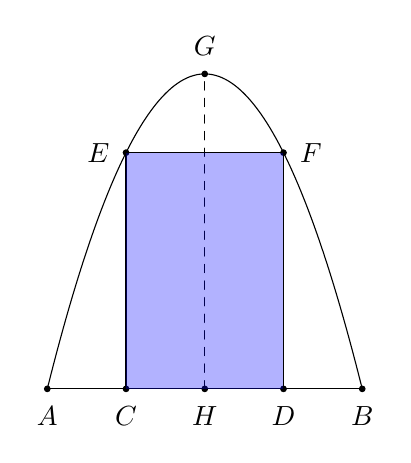
\begin{tikzpicture}[line join = round, line cap = round,>=stealth,scale=1]
	\path
	(0,0) coordinate(A)
	(4,0) coordinate(B)
	(1,0) coordinate(C)
	(2,0) coordinate(H)
	(3,0) coordinate(D)
	(1,3) coordinate(E)
	(3,3) coordinate(F)
	(2,4) coordinate(G)
	;
	\draw [black]
	plot[domain=0:4, samples=100] (\x, {-(\x)^2+4*(\x)});
	\draw (A)--(B) (D)--(F) (F)--(E) (E)--(C)
	;
	\draw[dashed] (H)--(G);
	\foreach \d/\g in{A/-90,C/-90,H/-90,D/-90,B/-90,E/180,F/0,G/90}\draw[fill=black](\d)circle(1pt)+(\g:0.35)node{$ \d $};
	\fill[blue,opacity=0.3] (1,0) rectangle (3,3);
	\end{tikzpicture}}
	\loigiai{
	\immini{Gắn hệ trục tọa độ $Oxy$ sao cho $ AB $ trùng $ Ox $, $ A $ trùng $ O $ khi đó parabol có đỉnh $ G(2;4) $ và	đi qua gốc tọa độ.\\
	Gọi phương trình của parabol là $ y=ax^2+bx+c $.\\ 
	Do đó ta có $ \left\{\begin{aligned}
	& c=0 \\
	& \dfrac{-b}{2\mathrm{a}}=2 \\
	& 2^2a+2b+c=4
\end{aligned}\right.\Leftrightarrow \left\{\begin{aligned}
	& a=-1 \\
	& b=4 \\
	& c=0.
\end{aligned}\right.$\\
	Nên phương trình parabol là $ y=f(x)=-x^2+4x $.\\ 
	Diện tích của cả cổng là
	\begin{eqnarray*}
	S=\displaystyle\int\limits_0^4(-x^2+4x)\mathrm{\,d}x=\left(-\dfrac{x^3}{3}+2x^2\right)\bigg|_0^4=\dfrac{32}{3}\approx 10{,}67\; (\mathrm{m}^2).
	\end{eqnarray*}
	Do vậy chiều cao $CF=DE=f(0{,}9)=2{,}79 $ (m),\\ $CD=4-2\cdot 0{,}9=2{,}2$ (m).\\ 
	Diện tích hai cánh cổng là $ S_{CDEF}=CD\cdot CF=6{,}138\approx 6{,}14 $ (m$^2$).\\ 
	Diện tích phần xiên hoa là $ S_{xh}=S-S_{CDEF}=10{,}67-6{,}14=4{,}53 $ (m$^2$).\\
	Nên tiền là hai cánh cổng là $ 6{,}14\cdot 1200000=7368000 $ (đồng) và tiền làm phần xiên hoa\\ là $4{,}53\cdot 900000=4077000 $ (đồng).\\
	Vậy tổng chi phí là $11445000$ đồng.
	}{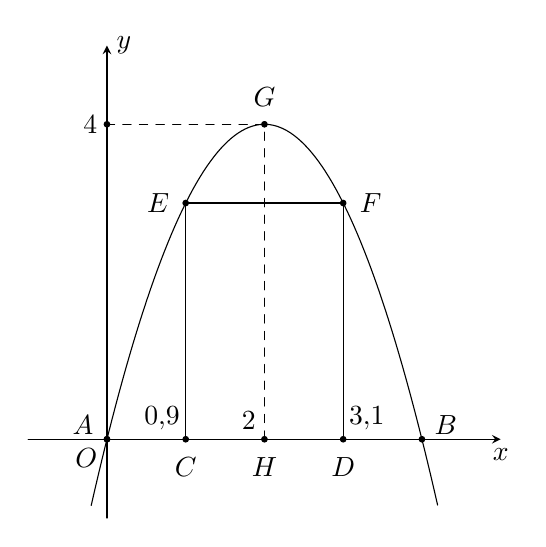
\begin{tikzpicture}[line join = round, line cap = round,>=stealth,scale=1]
	\draw[->] (-1,0) -- (5,0) node[below] {$ x $};
	\draw[->] (0,-1) -- (0,5) node[right] {$ y $};
	\path
	(0,0) coordinate(A)
	(4,0) coordinate(B)
	(1,0) coordinate(C)
	(2,0) coordinate(H)
	(3,0) coordinate(D)
	(1,3) coordinate(E)
	(3,3) coordinate(F)
	(2,4) coordinate(G)
	;
	\draw [black]
	plot[domain=-0.2:4.2, samples=100] (\x, {-(\x)^2+4*(\x)});
	\draw (A)--(B) (D)--(F) (F)--(E) (E)--(C)
	;
	\draw[dashed] (H)--(G) (2,0)--(2,4)--(0,4);
	\foreach \d/\g in{A/-210,C/-90,H/-90,D/-90,B/30,E/180,F/0,G/90}\draw[fill=black](\d)circle(1pt)+(\g:0.35)node{$ \d $};
	\draw[fill=black] (0,0) circle(1pt) node[below left]{$ O $} (0,4) circle(1pt)node[left]{$ 4 $} (0.7,0) node[above]{$ 0{,}9 $} (3.3,0) node[above]{$ 3{,}1 $} (1.8,0) node[above]{$ 2 $} 
	;
	%\fill[blue,opacity=0.3] (1,0) rectangle (3,3);
	\end{tikzpicture}} 
	}
\end{ex}
%%%=========HetCau_44=========%%%
%%==========Câu 45
\begin{ex}%[2H3K3-2]
	Trong không gian $ Oxyz $, cho hai đường thẳng $ d_1\colon\dfrac{x-3}{-1}=\dfrac{y-3}{-2}=\dfrac{z+2}{1} $; $ d_2\colon\dfrac{x-5}{-3}=\dfrac{y+1}{2}=\dfrac{z-2}{1} $ và mặt phẳng $ (P)\colon x+2y+3z-5=0 $. Đường thẳng vuông góc với $ (P) $, cắt $ d_1 $ và $ d_2 $ có phương trình là
	\choice
	{$\dfrac{x-2}{1}=\dfrac{y-3}{2}=\dfrac{z-1}{3}$}
	{$\dfrac{x-3}{1}=\dfrac{y-3}{2}=\dfrac{z+2}{3}$}
	{\True $ \dfrac{x-1}{1}=\dfrac{y+1}{2}=\dfrac{z}{3} $}
	{$ \dfrac{x-1}{3}=\dfrac{y+1}{2}=\dfrac{z}{1} $}
	\loigiai{
	Gọi $ \Delta $ là đường thẳng cần tìm. Gọi $ M=\Delta \cap d_1 $; $ N=\Delta \cap d_2 $.\\
	Vì $ M\in d_1 $ nên $ M(3-t; 3-2t; -2+t) $, $ N\in d_2 $ nên $ N(5-3s; -1+2s; 2+s) $.\\
	Ta có $ \overrightarrow{MN}= (2+t-3s; -4+2t+2s; 4-t+s) $, $ (P) $ có một vec tơ pháp tuyến là $ \vec{n}=(1; 2; 3) $.\\
	Vì $ \Delta \perp (P) $ nên $ \vec{n}, \overrightarrow{MN} $ cùng phương, do đó:
	\[\left\{\begin{aligned}
	& \dfrac{2+t-3s}{1}=\dfrac{-4+2t+2s}{2}\\
	& \dfrac{-4+2t+2s}{2}=\dfrac{4-t+s}{3}
	\end{aligned}\right.\Leftrightarrow \left\{\begin{aligned}
	& s=1 \\
	& t=2
	\end{aligned}\right.\Leftrightarrow \left\{\begin{aligned}
	& M(1; -1; 0) \\
	& N(2; 1; 3).
	\end{aligned}\right.\]
	Khi đó $ \Delta $ đi qua $ M $ và có một vectơ chỉ phương là $ \overrightarrow{MN}=(1; 2; 3) $.\\
	Do đó $ \Delta $ có phương trình chính tắc là $ \dfrac{x-1}{1}=\dfrac{y+1}{2}=\dfrac{z}{3} $.
	}
\end{ex}
%%%=========HetCau_45=========%%%
%%==========Câu 46
\begin{ex}%[2D1G2-2]
\immini{Cho hàm số $ y=f(x) $ có đồ thị $ y=f'(x) $ như hình vẽ bên. Đồ thị hàm số $ g(x)=  | 2f(x)- (x-1)^2 | $ có tối đa bao nhiêu điểm cực trị?
	\choice
	{$ 3 $}
	{\True $ 5 $}
	{$ 6 $}
	{$ 7 $}}{
	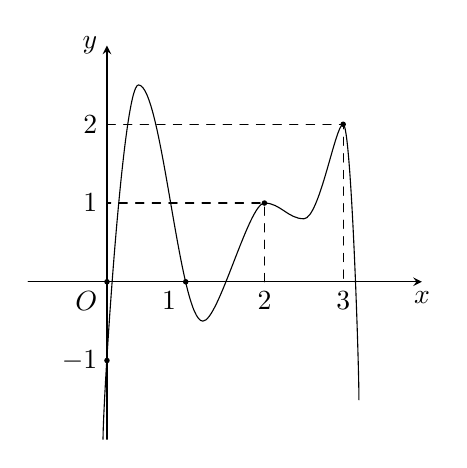
\begin{tikzpicture}[line join = round, line cap = round,>=stealth,scale=1]
		\draw[->] (-1,0)--(4,0)node[below]{$ x $};
		\draw[->] (0,-2)--(0,3)node[left]{$ y $};
		\draw[dashed] (2,0)node[below]{$ 2 $}--(2,1)--(0,1)node[left]{$ 1 $} (0,2)node[left]{$ 2 $}--(3,2)--(3,0)node[below]{$ 3 $} (1,0)node[below left]{$ 1 $} (0,0)node[below left]{$ O $}(0,-1)node[left]{$ -1 $};
		\draw (-0.05,-2)..controls+(90:0.5)and+(180:0.2)..(0.4,2.5)..controls+(0:0.3)and+(180:0.3)..(1.218,-0.5)..controls+(0:0.2)and+(180:0.2)..(2,1)..controls+(0:0.2)and+(180:0.2)..(2.5,0.8)..controls+(0:0.2)and+(180:0.1)..(3,2)..controls+(0:0.1)and+(90:0.5)..(3.2,-1.5);
		\foreach \diemx/\diemy in {1/0,2/1,3/2,0/-1,0/0}{\fill (\diemx,\diemy)circle(1pt);}
	\end{tikzpicture}
}
	\loigiai{
	Xét hàm số $ h(x)=2f(x)-(x-1)^2 $, ta có $ h'(x)=2f'(x)-2(x-1) $.\\
	 $ h'(x)=0\Leftrightarrow f'(x)=x-1\Leftrightarrow x=0\vee x=1\vee x=2\vee x=3 $.\\
	Bảng biến thiên
	\begin{center}
		
\begin{tikzpicture}[>=stealth]
			\tkzTabInit[nocadre=true,lgt=1.2,espcl=2,deltacl=0.5]
			{$x$/.7, $h'(x)$/.7, $h(x)$/2}
			{$-\infty$, $0$,$1$, $2$,$3$, $+\infty$}
			\tkzTabLine{,-,$0$,+,$0$,-,$0$,-,$0$,-,}
			\tkzTabVar{+/$+\infty$, -/, +/,R,R, -/$-\infty$}
		\end{tikzpicture}
	\end{center}
	Từ bảng biến thiên suy ra đồ thị hàm $ y=h(x) $ có $ 2 $ điểm cực trị. Đồ thị hàm số $ g(x)= | h(x) | $ nhận có tối đa $ 5 $ điểm cực trị.
	}
\end{ex}
%%%=========HetCau_46=========%%%
%%==========Câu 47
\begin{ex}%[2D2G6-3]
	Tập giá trị của $ x $ thỏa mãn $ \dfrac{2\cdot 9^x-3\cdot 6^x}{6^x-4^x}\le 2 (x\in \mathbb{R}) $ là $  (-\infty;a]\cup  (b;c ] $. Khi đó $ (a+b+c)! $ bằng
	\choice
	{$ 2 $}
	{$ 0 $}
	{\True $ 1 $}
	{$ 6 $}
	\loigiai{Điều kiện $ 6^x-4^x\ne 0\Leftrightarrow{\left(\dfrac{3}{2}\right)^x}\ne 1\Leftrightarrow x\ne 0 $.\\ 
	Khi đó $ \dfrac{2.9^x-3.6^x}{6^x-4^x}\le 2\Leftrightarrow \dfrac{2.\left(\dfrac{3}{2}\right)^{2x}-3.\left(\dfrac{3}{2}\right)^x}{\left(\dfrac{3}{2}\right)^x-1}\le 2 $.\\ 
	Đặt $ t=\left(\dfrac{3}{2}\right)^x $, $ t>0 $ ta được bất phương trình 
	\begin{eqnarray*}
	\dfrac{2t^2-3t}{t-1}\le 2\Leftrightarrow \dfrac{2t^2-5t+2}{t-1}\le 0 
	\Leftrightarrow \left[\begin{aligned}
	& t\le\dfrac{1}{2}\\
	& 1<t\le 2
	\end{aligned}\right.\Leftrightarrow \left[\begin{aligned}
	& \left(\dfrac{3}{2}\right)^x\le \dfrac{1}{2}\\
	& 1<\left(\dfrac{3}{2}\right)^x\le 2
	\end{aligned}\right.\Leftrightarrow \left[\begin{aligned}
	& x\le{\log_{\frac{3}{2}}}\dfrac{1}{2}\\
	& 0<x\le{\log_{\frac{3}{2}}}2.
	\end{aligned}\right.
	\end{eqnarray*}
	Vậy tập nghiệm của bất phương trình là $ \left(-\infty;\log_{\frac{3}{2}}\dfrac{1}{2}\right]\cup \left(0;\log_{\frac{3}{2}}2 \right] $.\\ 
	Suy ra $ a+b+c=\log_{\frac{3}{2}}\dfrac{1}{2}+\log_{\frac{3}{2}}2=0 $. Do đó $ (a+b+ct)!=1 $ 
	}
\end{ex}
%%%=========HetCau_47=========%%%
%%==========Câu 48
\begin{ex}%[2D3G3-1]
\immini{Cho hàm số $ y=x^4-3x^2+m $ có đồ thị $ (C_m) $, với $ m $ là tham số thực. Giả sử $ (C_m) $ cắt trục $ Ox $ tại bốn điểm phân biệt như hình vẽ. Gọi $ S_1 $, $ S_2 $, $ S_3 $ là diện tích các miền gạch chéo được cho trên hình vẽ. Giá trị của $ m $ để $ S_1+S_3=S_2 $ là
	\choice
	{$ -\dfrac{5}{2} $}
	{\True $ \dfrac{5}{4} $}
	{$ -\dfrac{5}{4} $}
	{$ \dfrac{5}{2} $}}{\begin{tikzpicture}[line join = round, line cap = round,>=stealth,scale=1]
	\def\f(#1){(#1)^4-3*(#1)^2+1.2}
	;
	\fill[pattern=north east lines,smooth] (-1.58,0) --
	plot[domain=-1.58:-0.68] (\x,{\f(\x)})
	-- (-0.68,0) -- cycle;
	\fill[pattern=north east lines,smooth] (-0.68,0) --
	plot[domain=-0.68:0.68] (\x,{\f(\x)})
	-- (0.68,0) -- cycle;
	\fill[pattern=north east lines,smooth] (0.68,0) --
	plot[domain=0.68:1.58] (\x,{\f(\x)})
	-- (1.58,0) -- cycle;
	\draw[fill=black]
	(1,0) node[above] {$ 1 $} circle (1pt) 
	(-1,0) node[above] {$ -1 $} circle (1pt) 
	(0,1) circle (1pt) 
	(2,0) node[above] {$ 2 $} circle (1pt) 
	(-2,0) node[above] {$ -2 $} circle (1pt) 
	;
	\path
	(-1.2,-0.4) node[fill=white,circle,inner sep=0pt]{$S_1$}
	(-0.2,0.5) node[fill=white,circle,inner sep=0pt]{$S_2$}
	(1.2,-0.35) node[fill=white,circle,inner sep=0pt]{$S_3$}
	(0.3,0.7) node[fill=white,circle,inner sep=0pt]{$1$}
	;
	\draw[->] (-3,0) -- (3,0) node[below] {$ x $};
	\draw[->] (0,-2) -- (0,3) node[right] {$ y $};
	\draw [black]
	plot[domain=-1.86:1.86, samples=100] (\x,{\f(\x)});
	\draw[fill=black] (0,0) circle(1pt) node[below left]{$ O $};
	\end{tikzpicture}}
	\loigiai{
	Gọi $ x_1 $ là nghiệm dương lớn nhất của phương trình $ x^4-3x^2+m=0 $, ta có $ m=-x_1^4+3x_1^2.\quad (1) $ \\
	Vì $ S_1+S_3=S_2 $ và $ S_1=S_3 $ nên $ S_2=2S_3 $ hay $ \displaystyle\int\limits_0^{x_1}f(x)\mathrm{\,d}x=0 $.\\
	Mà $ \displaystyle\int\limits_0^{x_1}f(x)\mathrm{\,d}x=\displaystyle\int\limits_0^{x_1} (x^4-3x^2+m)\mathrm{\,d}x= \left(\dfrac{x^5}{5}-x^3+mx\right) \bigg|_0^{x_1}=\dfrac{x_1^5}{5}-x_1^3+mx_1=x_1\left(\dfrac{x_1^4}{5}-x_1^2+m\right) $.\\
	Do đó, $ x_1\left(\dfrac{x_1^4}{5}-x_1^2+m\right)=0\Leftrightarrow \dfrac{x_1^4}{5}-x_1^2+m=0. \quad (2) $\\
	Từ $ (1) $ và $ (2) $, ta có phương trình $ \dfrac{x_1^4}{5}-x_1^2-x_1^4+3x_1^2=0\Leftrightarrow -4x_1^4+10x_1^2=0\Leftrightarrow x_1^2=\dfrac{5}{2} $.\\
	Vậy $ m=-x_1^4+3x_1^2=\dfrac{5}{4} $.
	}
\end{ex}
%%%=========HetCau_48=========%%%
%%==========Câu 49
\begin{ex}%[2D4G5-1]
	Cho số phức $ z $ thỏa mãn $ | z-1-i|+| z-3-2i |=\sqrt{5} $. Giá trị lớn nhất của $| z+2i | $ bằng
	\choice
	{$ 10 $}
	{\True $ 5 $}
	{$ \sqrt{10} $}
	{$ 2\sqrt{10} $}
	\loigiai{Gọi $ z=x+yi,(x,y\in \mathbb{R}) $.\\
	Khi đó $ | z-1-i |+| z-3-2i |=\sqrt{5}\Leftrightarrow |(x-1)+(y-1)i |+| (x-3)+(y-2)i|=\sqrt{5}.\quad(1) $ \\
	Trong mặt phẳng $ Oxy $, đặt $ A(1;1)$; $B(3;2) $; $ M(a;b) $.\\
	Khi đó số phức $ z $ thỏa mãn $ (1) $ là tập hợp điểm $ M(a;b) $ trên mặt phẳng hệ tọa độ $ Oxy $ thỏa mãn $ MA+MB=\sqrt{5} $.\\
	Mặt khác $ AB=\sqrt{(3-1)^2+(2-1)^2}=\sqrt{5} $ nên quỹ tích điểm $ M $ là đoạn thẳng $ AB $.\\
	Ta có $ | z+2i |=| a+(b+2)i | $. Đặt $ N(0;-2) $ thì $ | z+2i |=MN$.\\
	Gọi $ H $ là hình chiếu vuông góc của $ N $ trên đường thẳng $ AB $.	Phương trình $ AB\colon x-2y+1=0 $.\\
	Ta có $ H (-1;0) $ nên hai điểm $ A,B $ nằm cùng phía đối với $ H $.\\
	Ta có $\left\{\begin{aligned}
	& AN=\sqrt{1^2+3^2}=\sqrt{10}\\
	& BN=\sqrt{3^2+(2+2)^2}=5.
	\end{aligned}\right.$\\
	Vì $ M $ thuộc đoạn thẳng $ AB $ nên áp dụng tính chất đường xiên và hình chiếu ta có
	\[AN\le MN\le BN=5.\]
	Vậy giá trị lớn nhất của $ | z+2it| $ bằng $5$ đạt được khi $ M\equiv B(3;2) $, tức là $ z=3+2i $.
	}
\end{ex}
%%%=========HetCau_49=========%%%
%%==========Câu 50
\begin{ex}%[2H2G2-5]
Trong không gian với hệ tọa độ $ Oxyz $, cho mặt cầu $ (S)\colon (x-2)^2+(y-1)^2+(z-1)^2=9 $ và $ M(x_0;y_0;z_0)\in (S) $ sao cho $ A=x_0+2y_0+2z_0 $ đạt giá trị nhỏ nhất. Khi đó $ x_0+y_0+z_0 $ bằng
	\choice
	{$ 2 $}
	{\True $ -1 $}
	{$ -2 $}
	{$ 1 $}
	\loigiai{Ta có $ A=x_0+2y_0+2z_0\Leftrightarrow x_0+2y_0+2z_0-A=0 $ nên $ M\in (P)\colon x+2y+2z-A=0 $.\\
	Do đó điểm $ M $ là điểm chung của mặt cầu $ (S) $ với mặt phẳng $ (P) $.\\
	Mặt cầu $ (S) $ có tâm $ I(2;1;1) $ và bán kính $ R=3 $.\\
	Tồn tại điểm $ M $ khi và chỉ khi $ \mathrm{d}(I,(P))\le R\Leftrightarrow \dfrac{|6-A|}{3}\le 3\Leftrightarrow -3\le A\le 15 $.\\ 
	Do đó, với $ M $ thuộc mặt cầu $ (S) $ thì $ A=x_0+2y_0+2z_0\ge -3 $.\\
	Dấu đẳng thức xảy ra khi $ M $ là tiếp điểm của $ (P)\colon x+2y+2z+3=0 $ với $ (S) $ hay $ M $ là hình chiếu của $ I $ lên $ (P) $.\\ Suy ra $ M(x_0;y_0;z_0) $ thỏa: $ \left\{\begin{aligned}
	& x_0+2y_0+2z_0+3=0 \\
	& x_0=2+t \\
	& y_0=1+2t \\
	& z_0=1+2t
	\end{aligned}\right.\Leftrightarrow \left\{\begin{aligned}
	& t=-1 \\
	& x_0=1 \\
	& y_0=-1 \\
	& z_0=-1.
	\end{aligned}\right.$\\
	Vậy $ x_0+y_0+z_0=-1$.
	}
\end{ex}

\Closesolutionfile{ans}